% \documentclass[a4paper,twoside]{tufte-book}
\documentclass[a4paper,oneside,openany]{tufte-book}

\usepackage{xcolor} % for colour
\usepackage{lipsum} % just for sample text
\usepackage{pagecolor}
\usepackage[utf8]{inputenc}
\usepackage[english]{babel}
\usepackage[T1]{fontenc}
% \usepackage{chronology}
\usepackage{tikz}
\usepackage{graphicx}
\usepackage{array}









\newcommand\ytl[2]{
\parbox[b]{8em}{\hfill{\color{cyan}\bfseries\sffamily #1}~$\cdots\cdots$~}\makebox[0pt][c]{$\bullet$}\vrule\quad \parbox[c]{4.5cm}{\vspace{7pt}\color{red!40!black!80}\raggedright\sffamily #2.\\[7pt]}\\[-4pt]}


































\definecolor{chapco}{HTML}{4A96AD} % F52549
\definecolor{secColor}{HTML}{F52549}     % F62A00
\definecolor{subsecColor}{HTML}{F62A00} %FA6775
\definecolor{pBackColor}{HTML}{F5F3EE}  % ECECEA 6F6F6
            

\definecolor{myQuote}{HTML}{D50B53}
\definecolor{ptcbackground}{RGB}{212,237,252}
\definecolor{ptctitle}{RGB}{0,177,235}

% TOC
  \usepackage{titletoc}
  \usepackage{etoolbox}
  \setcounter{tocdepth}{2}



% add numbers to chapters, sections, subsections
\setcounter{secnumdepth}{2}

% chapter format
\titleformat{\chapter}%
  {\huge\rmfamily\itshape\color{chapco}}% format applied to label+text
  {\llap{\colorbox{chapco}{\parbox{1.5cm}{\hfill\itshape\huge\color{white}\thechapter}}}}% label
  {1em}% horizontal separation between label and title body
  {}% before the title body
  []% after the title body

% section format
\titleformat{\section}%
  {\normalfont\Large\itshape\color{secColor}}% format applied to label+text
  {\llap{\colorbox{secColor}{\parbox{1.5cm}{\hfill\color{white}\thesection}}}}% label
  {1em}% horizontal separation between label and title body
  {}% before the title body
  []% after the title body



% subsection format
\titleformat{\subsection}%
  {\normalfont\large\itshape\color{subsecColor}}% format applied to label+text
  {\llap{\colorbox{subsecColor}{\parbox{1.5cm}{\hfill\color{white}\thesubsection}}}}% label
  {1em}% horizontal separation between label and title body
  {}% before the title body
  []% after the title body





% Adjusts the size of the wheel:
\def\innerradius{1.8cm}
\def\outerradius{2.2cm}

% The main macro
\newcommand{\wheelchart}[1]{
    % Calculate total
    \pgfmathsetmacro{\totalnum}{0}
    \foreach \value/\colour/\name in {#1} {
        \pgfmathparse{\value+\totalnum}
        \global\let\totalnum=\pgfmathresult
    }

    \begin{tikzpicture}
    % The text in the center of the wheel
      \node[align=center,text width=2*\innerradius]{};

      % Calculate the thickness and the middle line of the wheel
      \pgfmathsetmacro{\wheelwidth}{\outerradius-\innerradius}
      \pgfmathsetmacro{\midradius}{(\outerradius+\innerradius)/2}

      % Rotate so we start from the top
      \begin{scope}[line width=\wheelwidth,rotate=90]

      % Loop through each value set. \cumnum keeps track of where we are in the wheel
      \pgfmathsetmacro{\cumnum}{0}
      \foreach \value/\colour/\name in {#1} {
            \pgfmathsetmacro{\newcumnum}{\cumnum + \value/\totalnum*360}

            % Calculate the percent value
            \pgfmathsetmacro{\percentage}{\value/\totalnum*100}
            % Calculate the mid angle of the colour segments to place the labels
            \pgfmathsetmacro{\midangle}{-(\cumnum+\newcumnum)/2}

            % This is necessary for the labels to align nicely
            \pgfmathparse{
               (-\midangle<5?"south":
                (-\midangle<85?"south west":
                 (-\midangle<105?"west":
                  (-\midangle<175?"north west":
                   (-\midangle<185?"north":
                    (-\midangle<265?"north east":
                     (-\midangle<275?"east":
                      (-\midangle<355?"south east":"south")
                     )
                    )
                   )
                  )
                 )
                )
               )
            } \edef\textanchor{\pgfmathresult}

            % Draw the color segments. Somehow, the \midrow units got lost, so we add 'pt' at the end. Not nice...
            \draw[\colour] (-\cumnum:\midradius pt) arc (-\cumnum:-(\newcumnum):\midradius pt);

            % Draw the data labels
            \node at (\midangle:\outerradius + 1ex) [inner sep=0pt, outer sep=0pt, ,anchor=\textanchor]{\name: \value\ (\pgfmathprintnumber{\percentage}\%)};

            % The 'spokes'
            \foreach \i in {0,...,\value} {
                \draw [gray,thin] (-\cumnum-\i/\totalnum*360:\innerradius) -- (-\cumnum-\i/\totalnum*360:\outerradius);
            }

            % Set the old cumulated angle to the new value
            \global\let\cumnum=\newcumnum
        }

      \end{scope}
      \draw[gray] (0,0) circle (\outerradius) circle (\innerradius);
    \end{tikzpicture}
}







































% \setlength{\parindent}{2em}
\setlength{\parskip}{1em}





\title{Reference \& Certify Token}
\author{foundation@rctoken.com \\ verson 0.3.2}















\begin{document}
% \pagecolor{pBackColor}
\maketitle
\tableofcontents

































%----------------------------------

\chapter{Background and Concept of Design}

The popularity of the Internet and smart phones has brought us into the We-media era (We-media Era). According to the statistics, the updating amount of only more than 50 microblogging, blog sites has reached more than 200 million/day. This is a time when everyone can participate and everyone is creating. A computer and a cell phone can become the tool of creation; one can easily become a star online with a beautiful photo and a witty humor can turn into a network buzzword. The fast dissemination of information is overwhelming. However, here follows the issue of intellectual property protection. The reproducibility of Internet files speeds up the dissemination of information, while also increasing the difficulty of property rights protection. The works on the Internet will soon be copied by others, and then spread, and sometimes it is difficult to find the original author of the work. This is not only infringement of intellectual property rights and damage to the original author's rights and interests, it also dampens the authors' enthusiasm to further create better works. If there is a program to give the creator corresponding reward according to the influence of his works at the same time of protecting the creative results, it will ignite the passion of innovation and promote the continuous cultural prosperity in the We-media era.    






The birth and application of blockchain brings hope for this. Proposed by Satoshi Nakamoto in "Bitcoin: A Peer-to-Peer Electronic Cash System"\sidenote{Nakamoto, Satoshi (October 2008). "Bitcoin: A Peer-to-Peer Electronic Cash System" bitcoin.org. Retrieved 28 April 2014.},       whitepaper of Bitcoin, in October, 2008, it is an intelligent peer-to-peer network to identify, transmit and record information using distributed database. The blockchain technology, based on decentralized peer-to-peer network, combines cryptography principle, the time series data and the consensus mechanism to ensure the continuity and persistence of the nodes in the distributed database with open source software, so that the information that can be verified and traced back immediately will be difficult to tamper and cannot be shielded, thus creating a set of private, efficient and secure shared value system \sidenote{Iansiti, Marco; Lakhani, Karim R. "The Truth About Blockchain". Harvard Business Review (Harvard University). January 2017 [2017-01-17].}.      The system is also known as the Value Internet, which can transmit virtual currency, implement smart contracts automatically, etc. without requiring third party participation and review of any centralization agency. Since its inception, the value of the blockchain technology itself has been discovered and recognized continuously \sidenote{Popper, Nathan (2016-05-21). "A Venture Fund With Plenty of Virtual Capital, but No Capitalist". New York Times. Retrieved 2016-05-23.}      \sidenote{Morris, David Z. (2016-05-15). "Leaderless, Blockchain-Based Venture Capital Fund Raises \$100 Million, And Counting". Fortune. Retrieved 2016-05-23.}  .         In the case of Bitcoin, for example, the first transaction recorded was that a programmer named Laszlo Hanyecz in the United States bought two pizza with 10,000 BTC on May 22, 2010. By May 22, 2017, the same amount of Bitcoin was valued at about \$ 22.89 million, appreciating by about 1 million times. What lies behind is more than the favor of capital, rather, it is the embodiment of the value of the blockchain itself.




The combination of the blockchain with innovation and creation has epoch-making significance, which is also the concept of design of the proof chain project embodied in the following aspects:


\begin{itemize}
  \item The proof chain uses the infinity of the address space to cover every piece of work for each person. In the RCT network, each piece of work, such as a microblogging, a blog, a picture, a music, a video, a paper, a patent, etc., can get a wallet address for its unified resource locator (URL) through Hash calculation. The key to the wallet belongs to the creator himself to ensure his ownership.
  \item The proof chain uses the "transaction history" of the blockchain to record the citation relationship between the works. The creator adds "reference" in the process of making the wallet address, namely, listing the wallet address of other works that are quoted, reproduced, and forwarded in creating the work to establish the proof network. The records that have been repeatedly confirmed in the blockchain will be difficult to overturn, and the difficulty and the number of confirmations will increase exponentially, which will ensure the reliability of the proof relationship.
  \item The blockchain adopts the unique PoW + PoI consensus mechanism to award RCT tokens for excellent works. For RCT tokens of each block, 60\% will be given to miners and 40\% will be given to the excellent works according to the influence of the work in the proof relationship network. This ensures that the creator as "intellectual exporter" and the miner as "technical service exporter" have a considerable income to encourage creators to create more influential works.
  \item The proof chain, relying on the open and transparent features of the distributed account books of the blockchain, makes it possible for the public to supervise the miners and creators. The transactions and proof relationship in the proof chain are stored on different nodes in the form of blockchains, so everyone can go back and check the historical records.



\end{itemize}































%--------------------------------------


\chapter{Our Mission And Team}

\section{Our Mission}

\begin{quote}
\textsf{\color{myQuote}{\textbf{\textit{\Large Protect each and every intellectual creation, encourage innovation and creation and help everyone realize his dream through creation.}}}}
\end{quote}


The popularity of the Internet and mobile Internet enables everyone to become a good creator. The team of the proof chain is committed to using blockchain technology to help each creator protect the results of intellectual labor, help each creator to benefit from his work, encourage every creator to create better works and ultimately help each creator to achieve his dream through innovative creation.



\section{Team}
Table \ref{tab_teamMembers}.







\begin{table}[ht]
\centering
\caption{Team Members}
\label{tab_teamMembers}
\begin{tabular}{ l | l }
     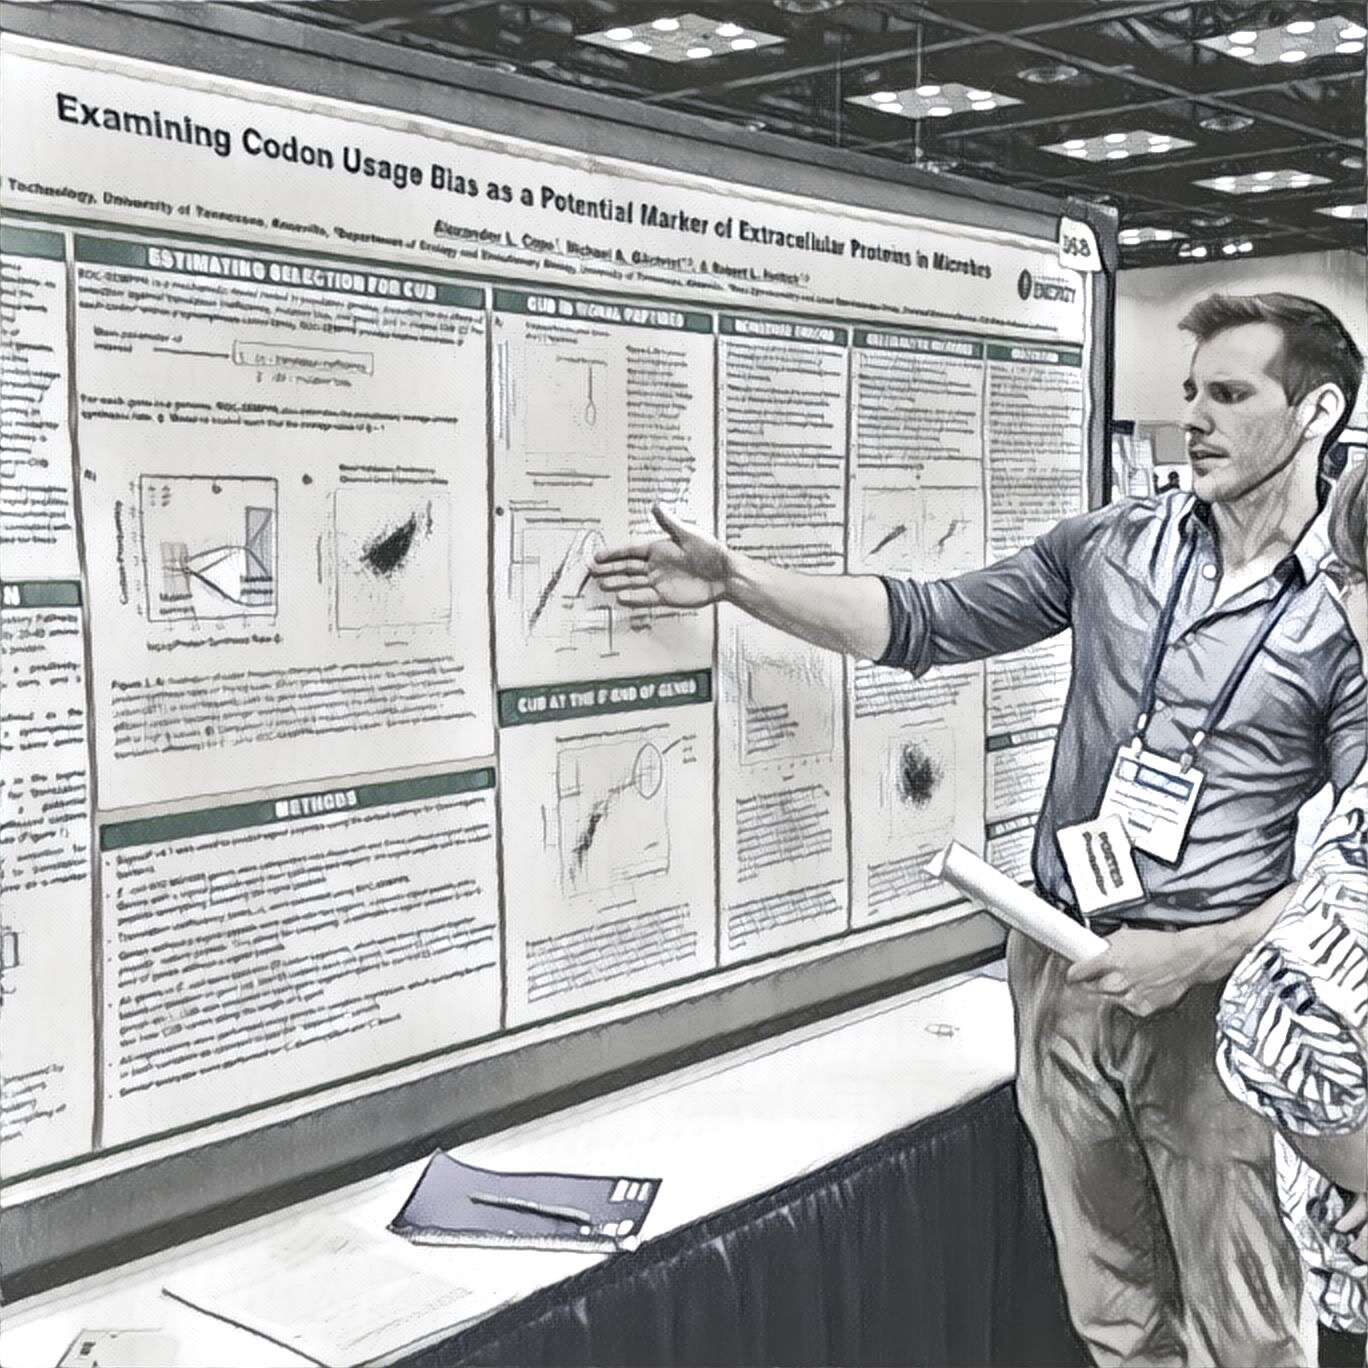
\includegraphics[width=30mm]{fig/p2} & \begin{minipage}{40em}
  \emph{Alexander Cope} \\ received his B.S. in Mathematics and Computer Science from \emph{Centre College} in 2015. He is currently a Ph.D. student at the \emph{University of Tennessee, Knoxville} and \emph{Oak Ridge National Laboratory}. Working in the labs of Michael Gilchrist and Robert Hettich, his current research interest is the development of computational models to analyze huge data sets. Prior to his Ph.D. work, his projects included sports analytics, computational fluid dynamics, and database development.
\end{minipage}\\
     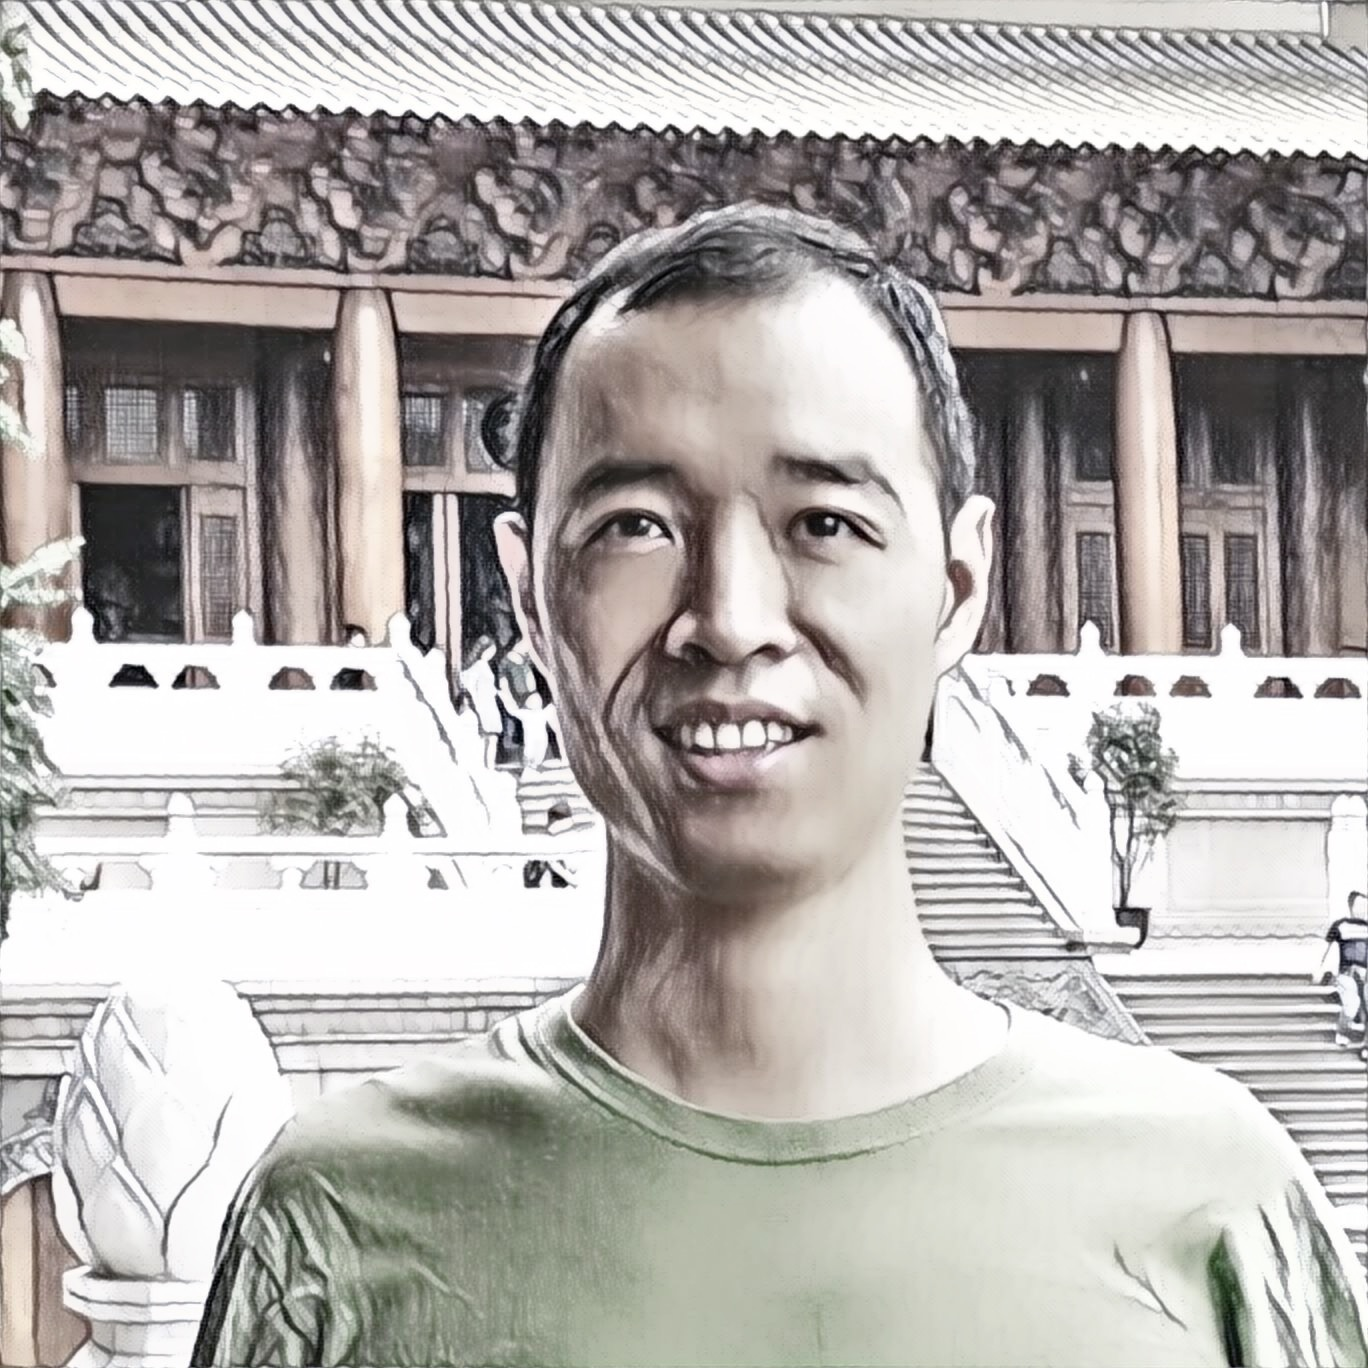
\includegraphics[width=30mm]{fig/p4} &\begin{minipage}{40em}
  \emph{Jason Lian} \\ received his Ph.D. degree at \emph{Shanghai Jiao Tong University}. He is also a cryptocurrency \& blockchain enthusiast. As a former Senior Data Mining Engineer at \emph{Holaverse}, he worked on mobile internet big data datamining and recommendation algorithm development. He was involved in blockchain field since 2013 and joined RCT in 2017, responsible for the development of the infrastructure of RCT blockchain.
\end{minipage} \\
      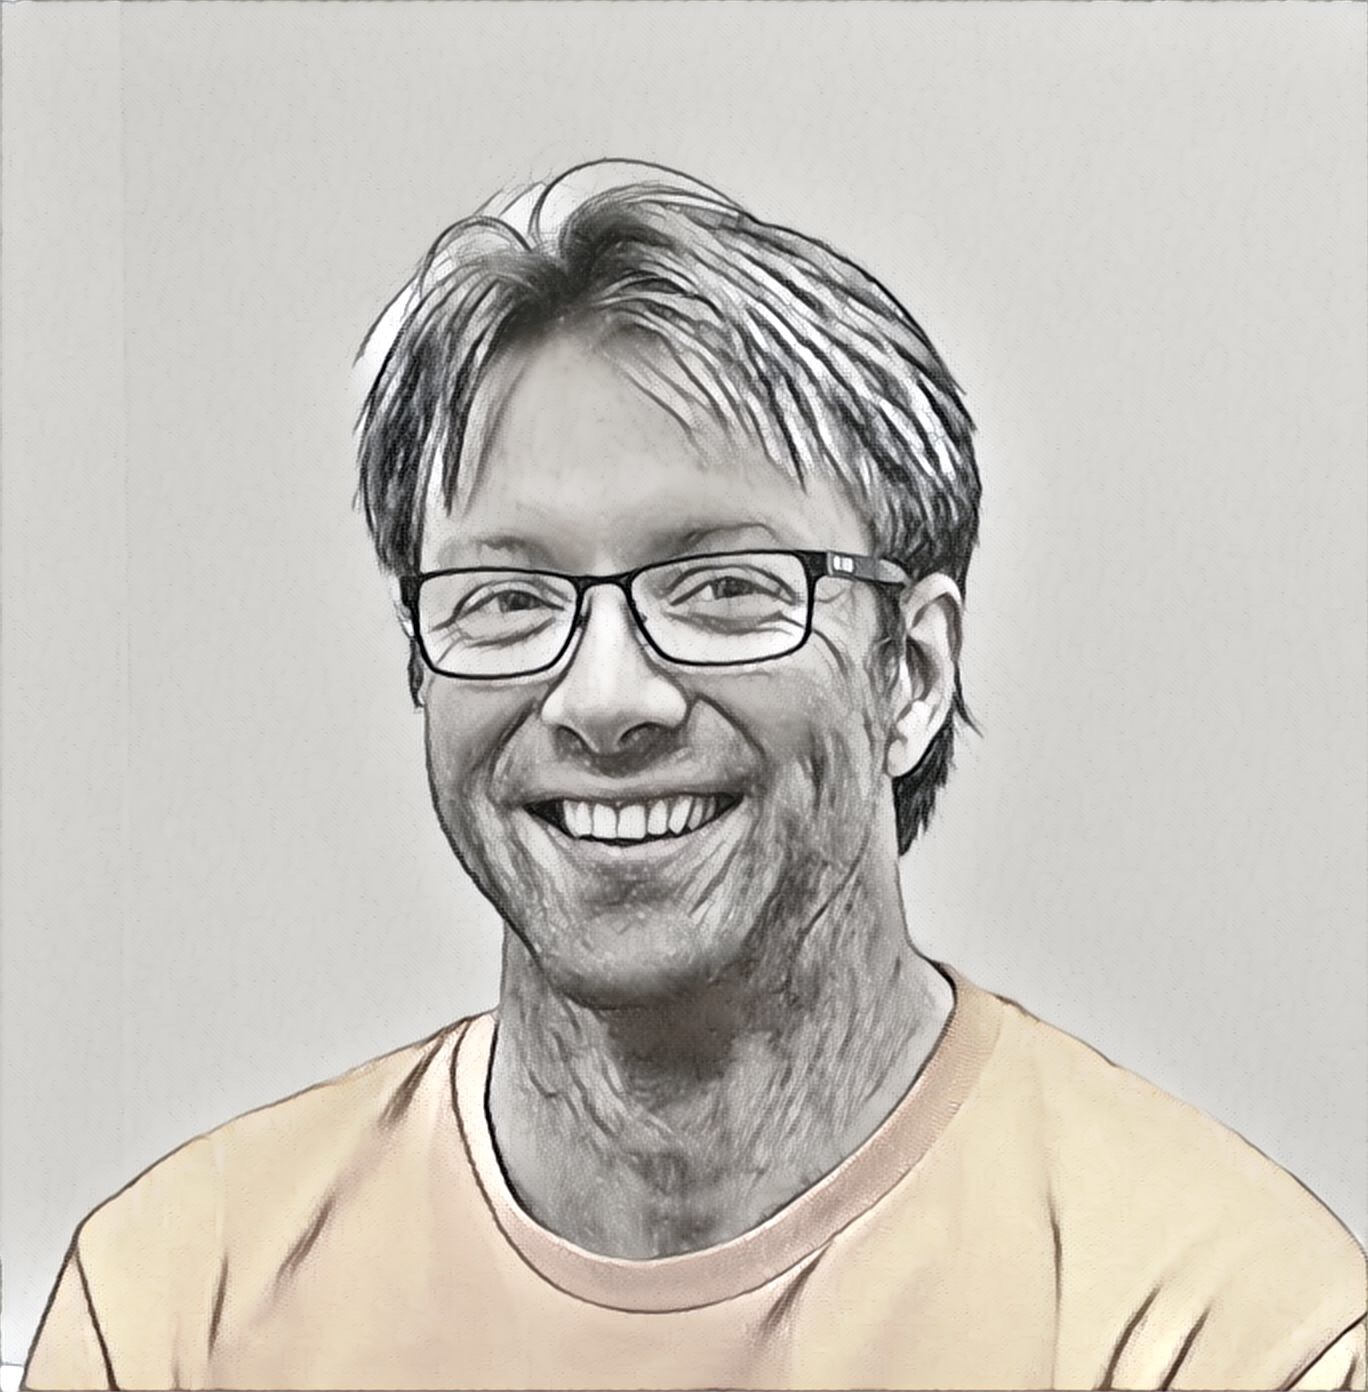
\includegraphics[width=30mm]{fig/p3}     &\begin{minipage}{40em}
  \emph{Stephen Grady} \\ received his B.S. from \emph{University of Arkansas} in 2012.  He is currently a Ph.D candidate at the \emph{University of Tennessee, Knoxville} and \emph{Oak Ridge National Laboratory}.  Under the guidance of Dr. Michael A. Langston, his current research interests are dominating set, graph algorithms, applications and implementations. Prior to his Ph.D. work, his projects included statistical and nonlinear physics and neuroscience.
\end{minipage} \\
     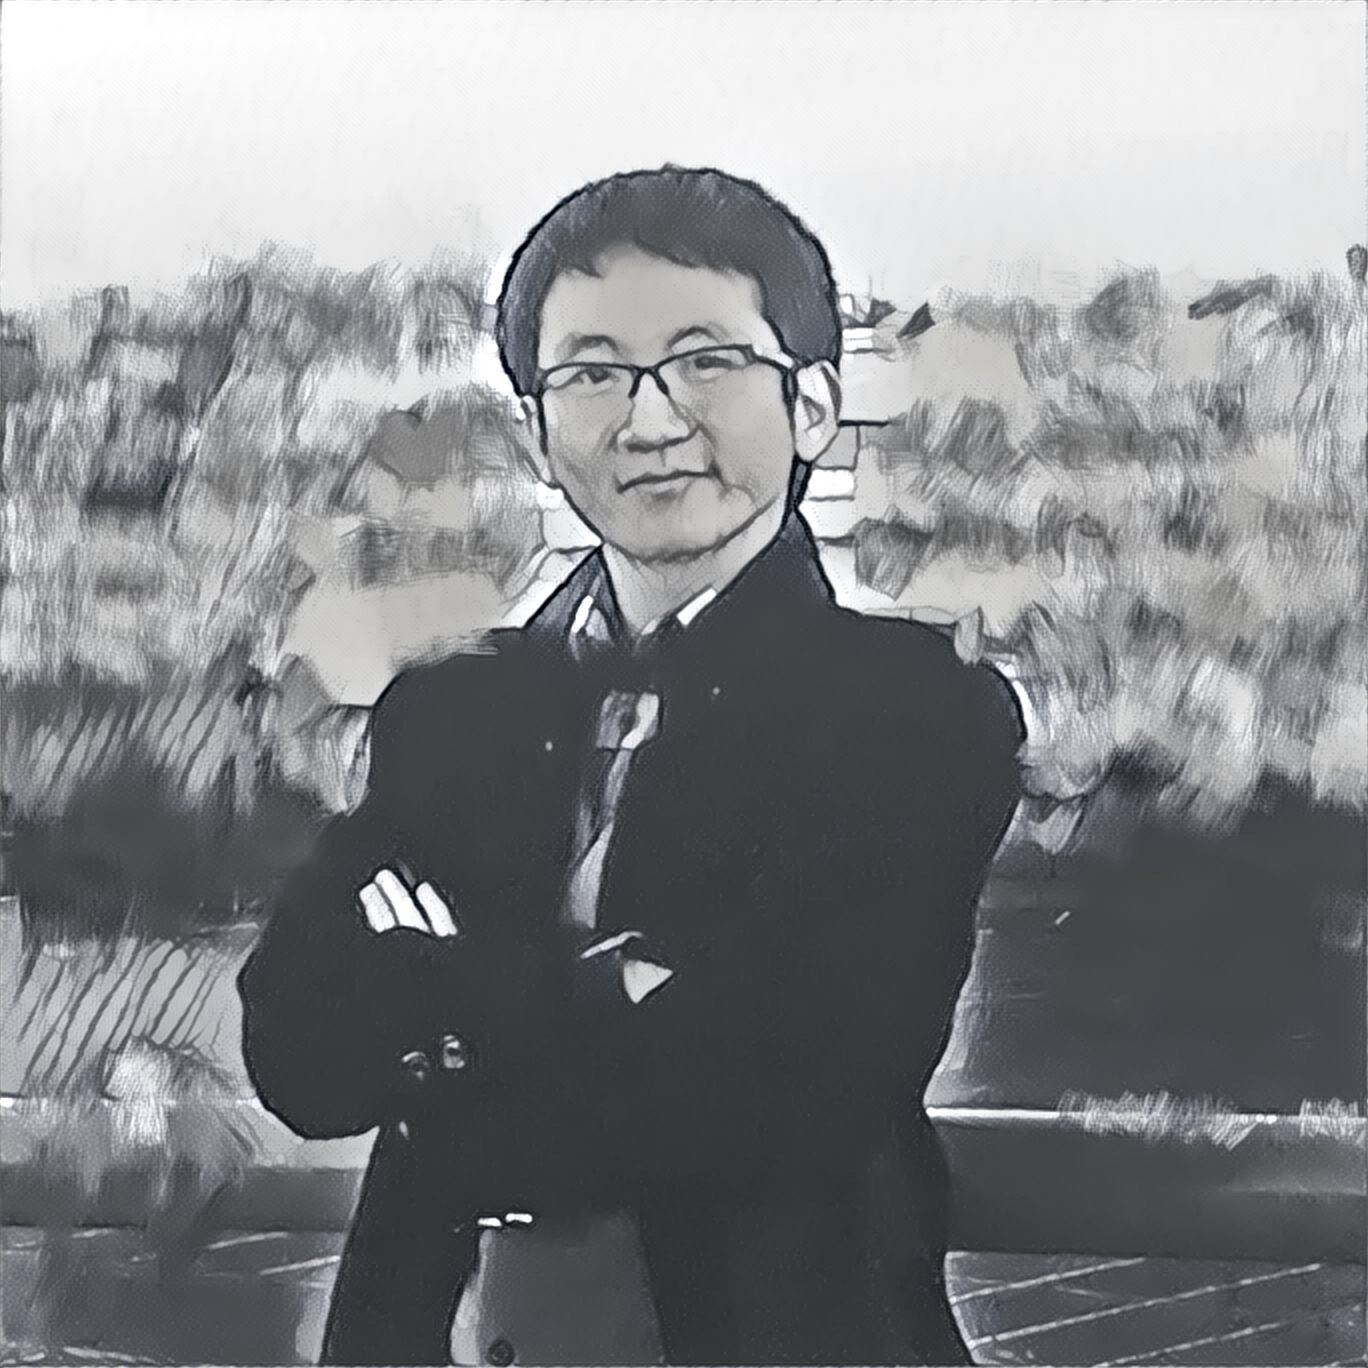
\includegraphics[width=30mm]{fig/p1} & \begin{minipage}{40em}
  \emph{Yaojin Sun} \\ received his B.S. degree at \emph{Shanghai Jiao Tong University}. He is currently a Ph.D. candidate at \emph{Haslam College of Business, the University of Tennessee}. Guided by Dr. Hamparsum Bozdogan, his current research interests include machine learning algorithms, statistical information theory and handling large data sets for decision making. He was involved in blockchain field since 2015 and joined RCT project in 2017, responsible for the development of consensus algorithm concerning blockchain infrastructure.
\end{minipage}
\end{tabular}
\end{table}

























%--------------------------------------


\chapter{Innovation of the Citation Chain}



\section{Blockchain Design}

We introduce a decentralized assessment method based on the blockchain to quantify or even conduct real-time assessment for the works published.



In RCT network, we want to expand the definition of "citation". The work will not be limited in terms of the format and form, and it can be an academic article, a picture, a video or even just a passage. And "citation" refers not only to the index relationship between academic papers, it can also be a citation to the author of the work, and even citation of each of the pictures by an article. In the blockchain, we use "Transaction" to bear "citation".


The citation of the work embodies the value of the work itself. A work cited by more accounts shows that it has a higher value. Similarly, a work cited by another work with a higher value also represents a higher value. This idea is widely used in activities such as page rankings.




\section{Incentive Mechanism}


\subsection{Proof of Importance (PoI)}

Proof of Importance (PoI) was first applied in the New Economy Movement (NEM). Because the transaction information for each account is public to the entire network, a large transaction matrix can be constructed based on past transaction history. Each account is calculated with a corresponding importance score, and an account with a high importance score is more likely to gain the reward of the next block. By introducing the NCDawareRank algorithm, the importance score of the eligible account in the network is calculated.





In the blockchain network, there may be tens of millions of accounts with the number of transactions even in billions. An algorithm based on similar PageRank and NCDawareRank results in an exponential rise in the consumption of computer memory. However, NEM bypasses the problem of computer memory consumption by increasing the filtering conditions, for example, the amount of transaction must be large enough; the blocked generated in the past 30 days will be calculated in the blockchain, etc. By adding filtering conditions of the account, there are only a few hundred accounts that are included in the calculation.


The application of NEM to PoI is feasible in the algorithm, but it is problematic for the evaluation of the value based on academic citation. Due to the limit of the amount of the transaction, the account balance itself can also affect the academic value of the work. This is contrary to the idea of decentralization.



In order to solve both the problem of decentralization and computer memory consumption, we introduce the mathematical model of "Random Walk" in order to balance the value judgment and the normal operation of the blockchain network.

\subsection{Random Walk Model}



\begin{marginfigure}
  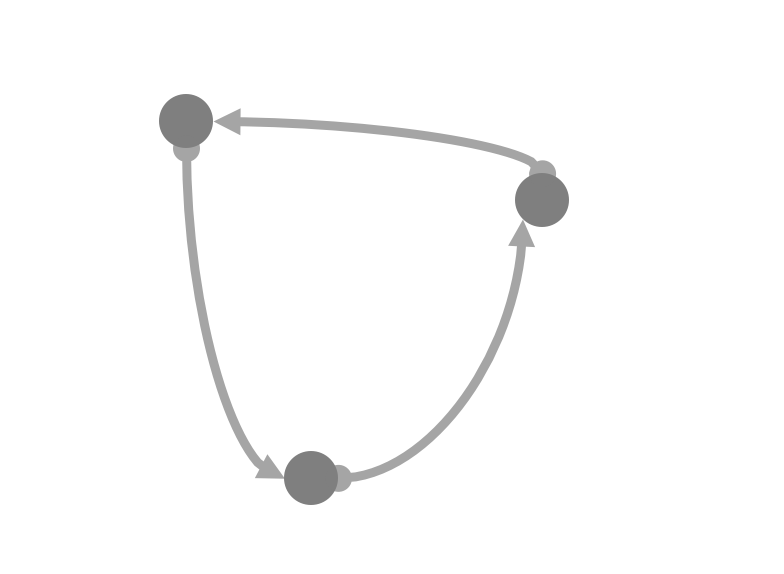
\includegraphics[width=\textwidth]{fig/cirC.png}
  \caption{Circular citation}
\end{marginfigure}



\begin{marginfigure}
  
\includegraphics[width=\textwidth]{fig/selfC.png}
  \caption{Self-citation}
\end{marginfigure}



The problem that Random Walk intends to solve is to achieve value judgment based on the citation relationship between the accounts entirely  without significantly increasing memory consumption. The following figure shows a hypothetical academic citation network. In the blockchain, the concept of “citation" is more flexible than the current generic concept, and may not be limited to time. If a drunk jumps and walks randomly in the network with one jump every time, the direction of jump must be the direction of citation. With limited steps, the place where the drunk finally stays is the location that has significant value for this network. 




Because in the citation chain network, the implementation of "citation" is neither limited to time nor limited to works, so there will be "self-citation" and "circular citation". In the case of circular citation and self- citation, the Random Walk Model is easily used by miners to reduce the difficulty of searching, but cannot achieve the reward for high-value works. For this type of problem, we add a restrictive condition that each account in the Citation Chain can appear at most once. In this case, the search difficulty will be maintained in a relatively stable degree.

\begin{figure}
  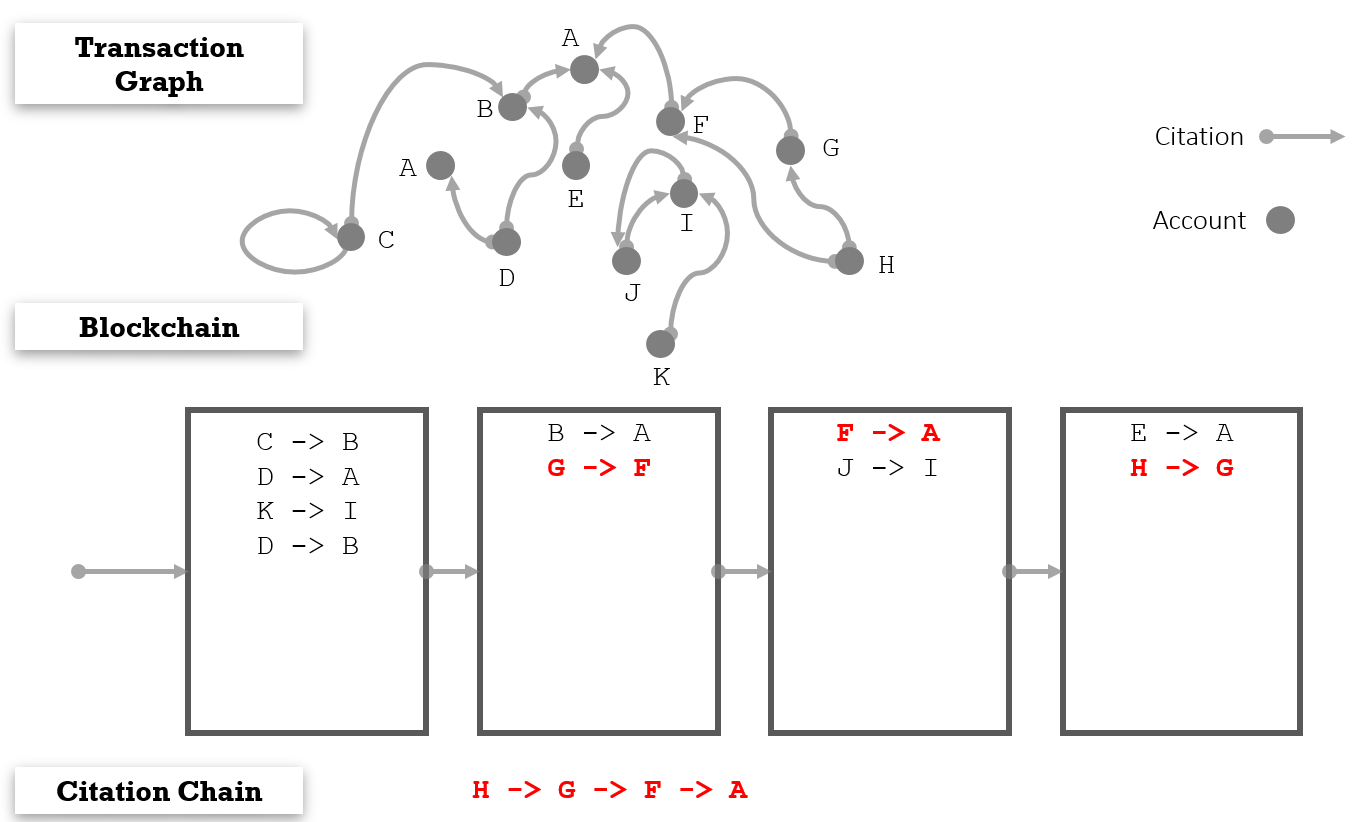
\includegraphics[width=\textwidth]{fig/citeG.png}
  \caption{Transaction graph, blockchain and citation chain}
\end{figure}



The information on the blockchain is very valuable and expensive. And too many steps in Random Walk will not be accepted; otherwise the corresponding block size will increase significantly, even increased to the extent that no miners have enough time to verify. The current number of Random Walk is at most 8 steps and at least 1 step. In the above figure, the citation chain generated by Random Walk contains 3 steps.


In order to encourage miners to carry out Random Walk operations as much as possible (i.e., to find the most valuable works in the blockchain), the number of Random Walk will have impact on the difficulty of the whole block.


\[
f(x)=1-\frac{1}{2(1+e^{x-\overline{x}})}
\]


\begin{itemize}
  \item $\overline{x}$: the average number of steps of Random Walk in past blocks
  \item $x$: number of steps for Random Walk in the current block
  \item $f$: current difficulty coefficient
\end{itemize}















\begin{marginfigure}
  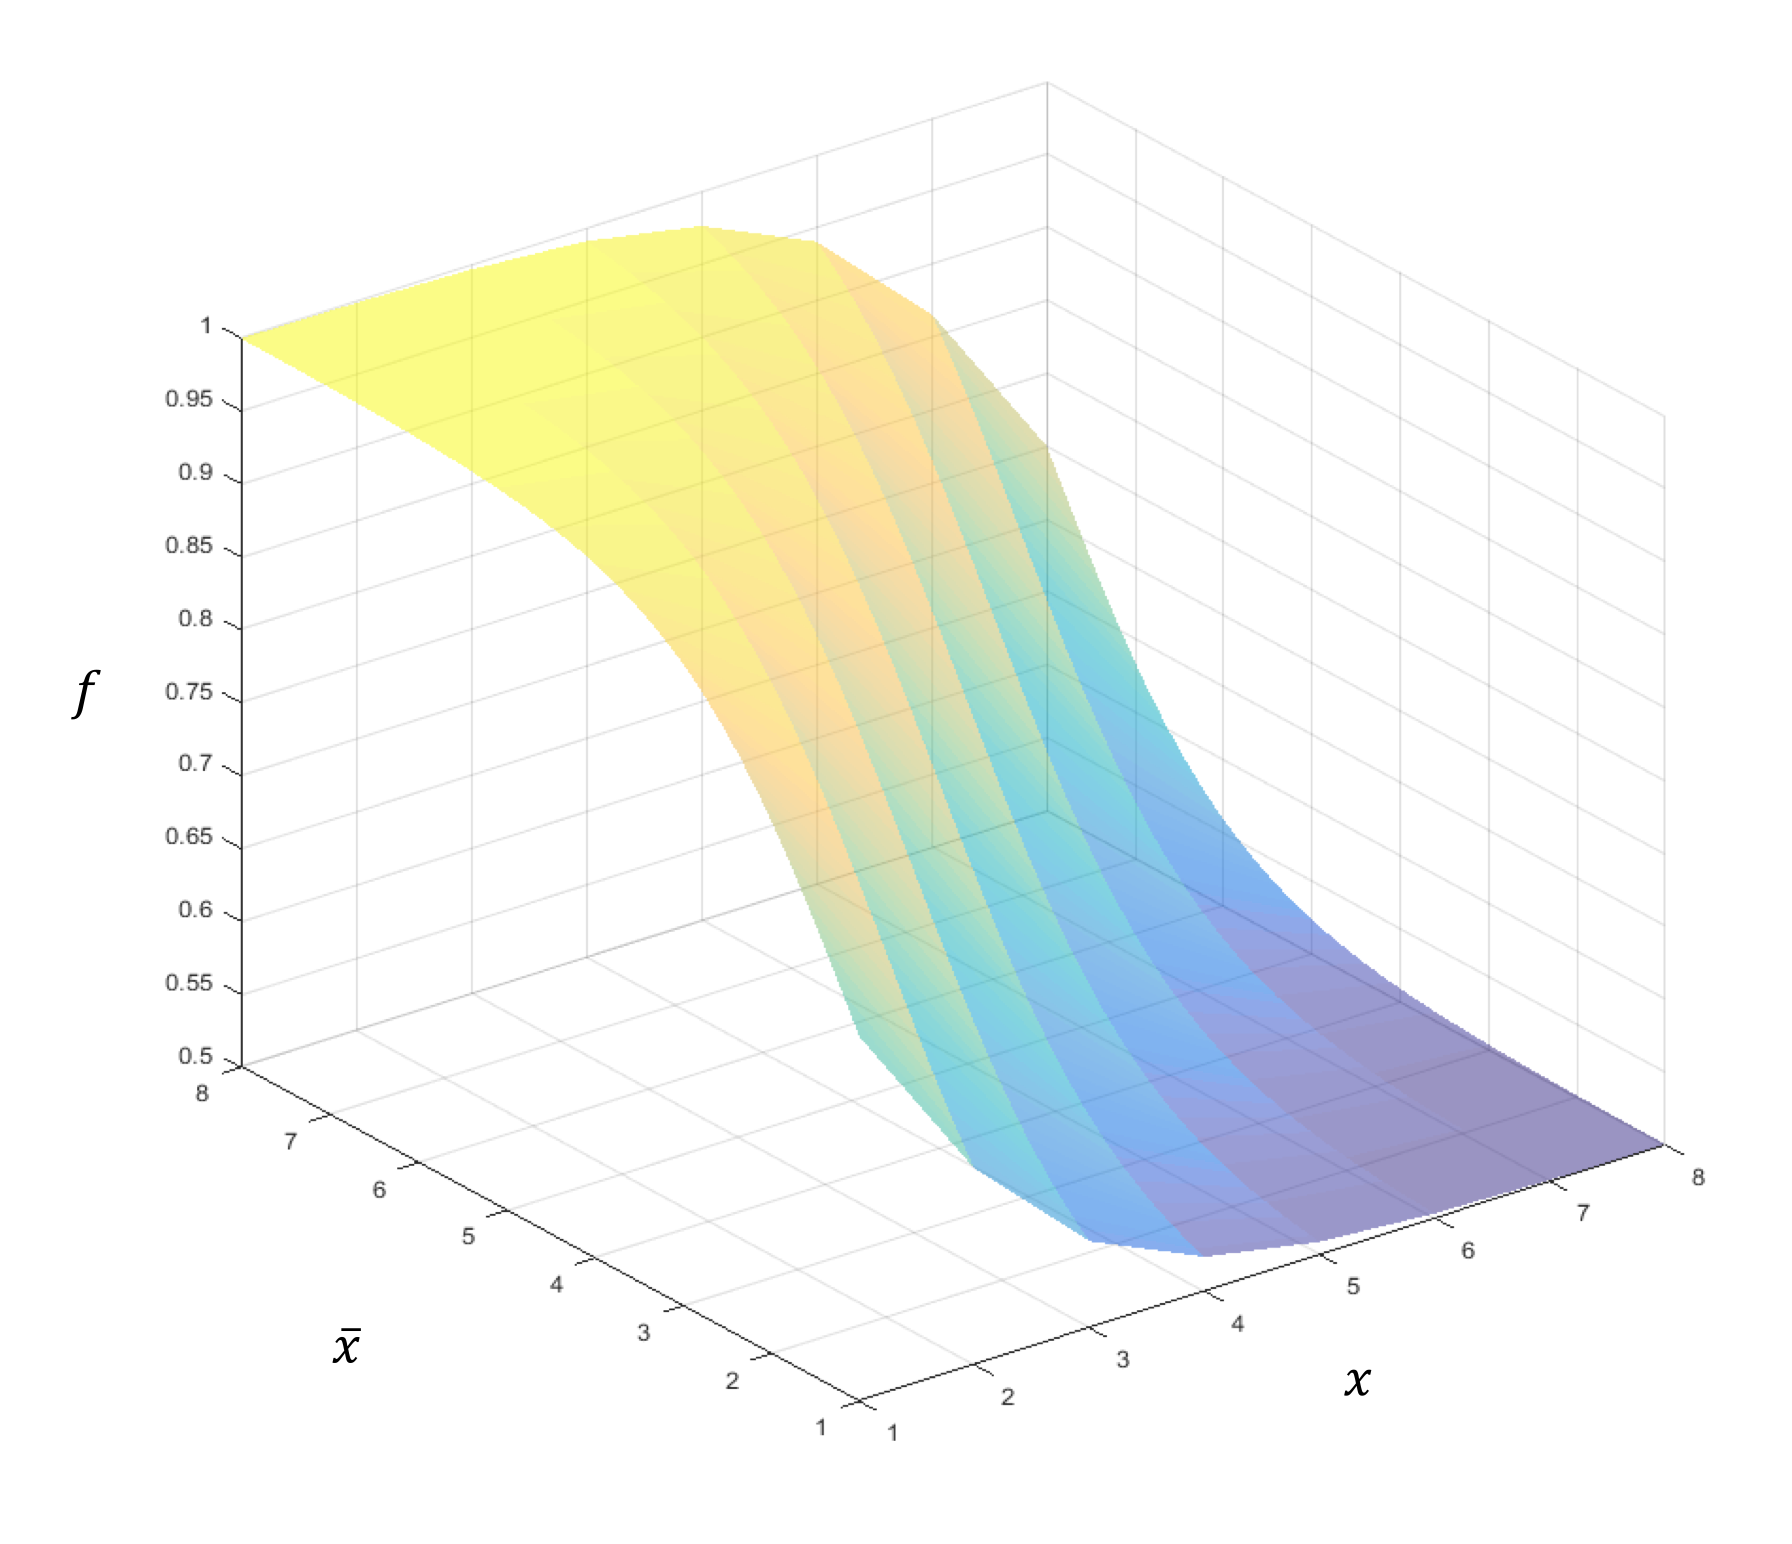
\includegraphics[width=\textwidth]{fig/f1.png}
  \caption{The surface of $f(x)$}
\end{marginfigure}

\begin{marginfigure}
  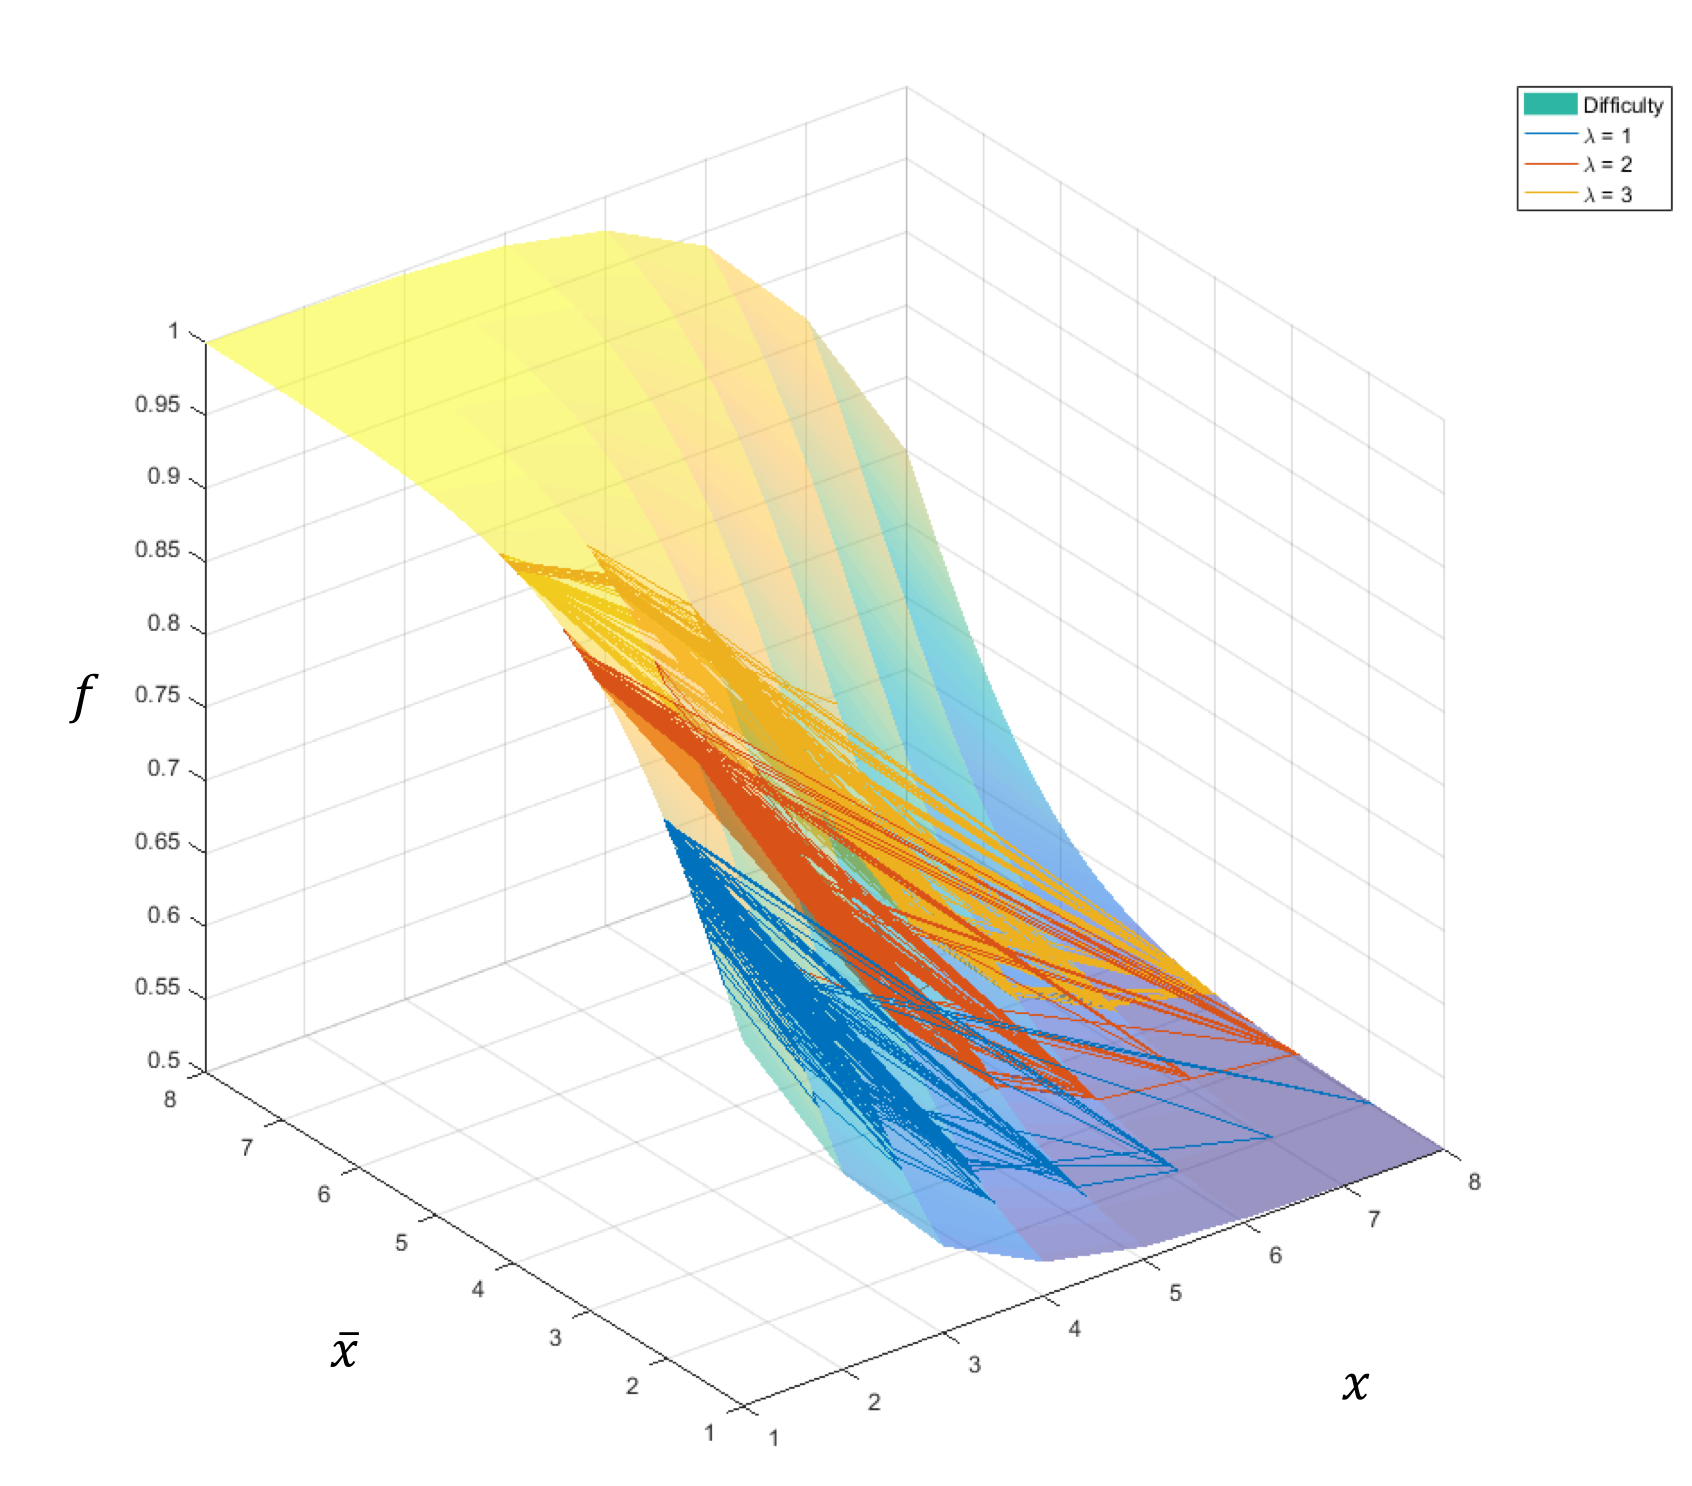
\includegraphics[width=\textwidth]{fig/f2.png}
  \caption{The surface of $f(x)$ with simulation results}
\end{marginfigure}








\section{Difficulty Calculation and Confirmation of Block}


Bitcoin and other current mainstream currencies are mainly based on PoW for the construction and confirmation of the block. We will combine PoI and PoW to achieve double protection for miners and content providers.



In the previous section, we have been able to get a difficulty coefficient f through random surfer. In the new block confirmation, a portion of the PoW still uses the SHA256 algorithm to calculate the zero character matching the times, and the second part, the specific hash value must be greater than the difficulty coefficient f. We note that after the introduction of the Random Walk Model, if no Random Walk is attempted (i.e., the number of steps is 1), the difficulty coefficient will be close to $1$, and if the number of steps of the citation chain reaches 8, the difficulty coefficient $f$ will be close to $0.5$. The two corresponds to about 50\% of the calculation of the difference.



For an honest miner, he will, as far as possible, \emph{go back to the entire block as much as possible and find all possible citation chains to reduce the corresponding difficulty coefficient}. With the increase in the number of blocks, the difficulty of search will increase. When the difficulty of the search increases to a certain extent, the miner will give up the search (he will search only 1 corresponding step in extreme cases) and turn into PoW calculation. This result will reduce the average length of the citation chain, and in this case the advantage of search is explored again, and the miner will search more blocks to obtain a reduction in the difficulty coefficient.


After each block is confirmed, there will be a certain amount of reward provided. The total award is divided into two parts: the first part is the miner (60\%) who completed the current block, and the second part is the final account (40\%) cited by the citation chain, which is identified as a work with important value in the current block.


\begin{figure}
% Usage: \wheelchart{<value1>/<colour1>/<label1>, ...}
\wheelchart{60/RoyalBlue/PoW,  40/WildStrawberry/PoI}
\caption{Consensus mechanism. (Unit: Percent)}
\end{figure}


















































%--------------------------------------

\chapter{Possible Attacks and Solutions}


\section{Sybil Attack}

Sybil Attack is the most common problem in blockchain design. For a completely PoW-based Bitcoin and other blockchain system, the premise of a witch attack is the grasp more than half of the computing power of the entire network. In the RCT, sybil attack for a certain block not only needs have sufficient computing power, but also requires the ability to trace back the entire blockchain. Because the starting position of the Random Walk is randomly determined by the previous block, the corresponding attack difficulty is no less than the PoW-based blockchain network.




\section{Low-value Works}

\begin{marginfigure}
  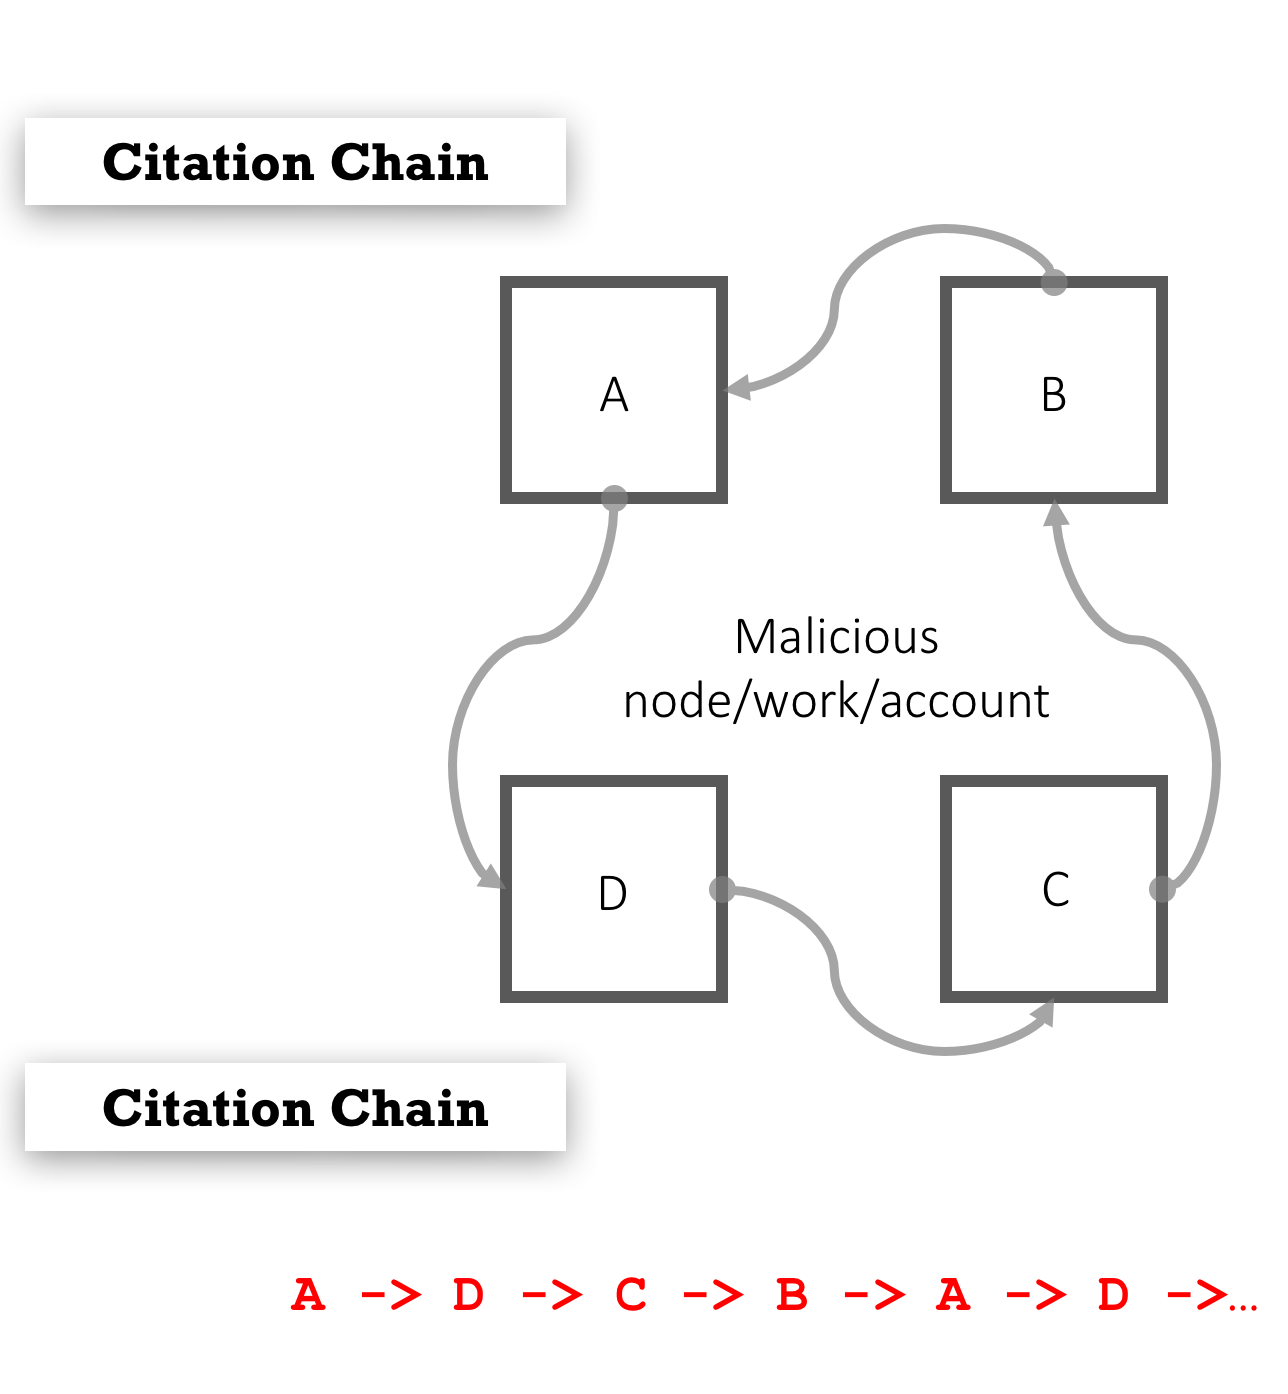
\includegraphics[width=\textwidth]{fig/loopA.png}
  \caption{Loop Attack}
\end{marginfigure}



\begin{marginfigure}
  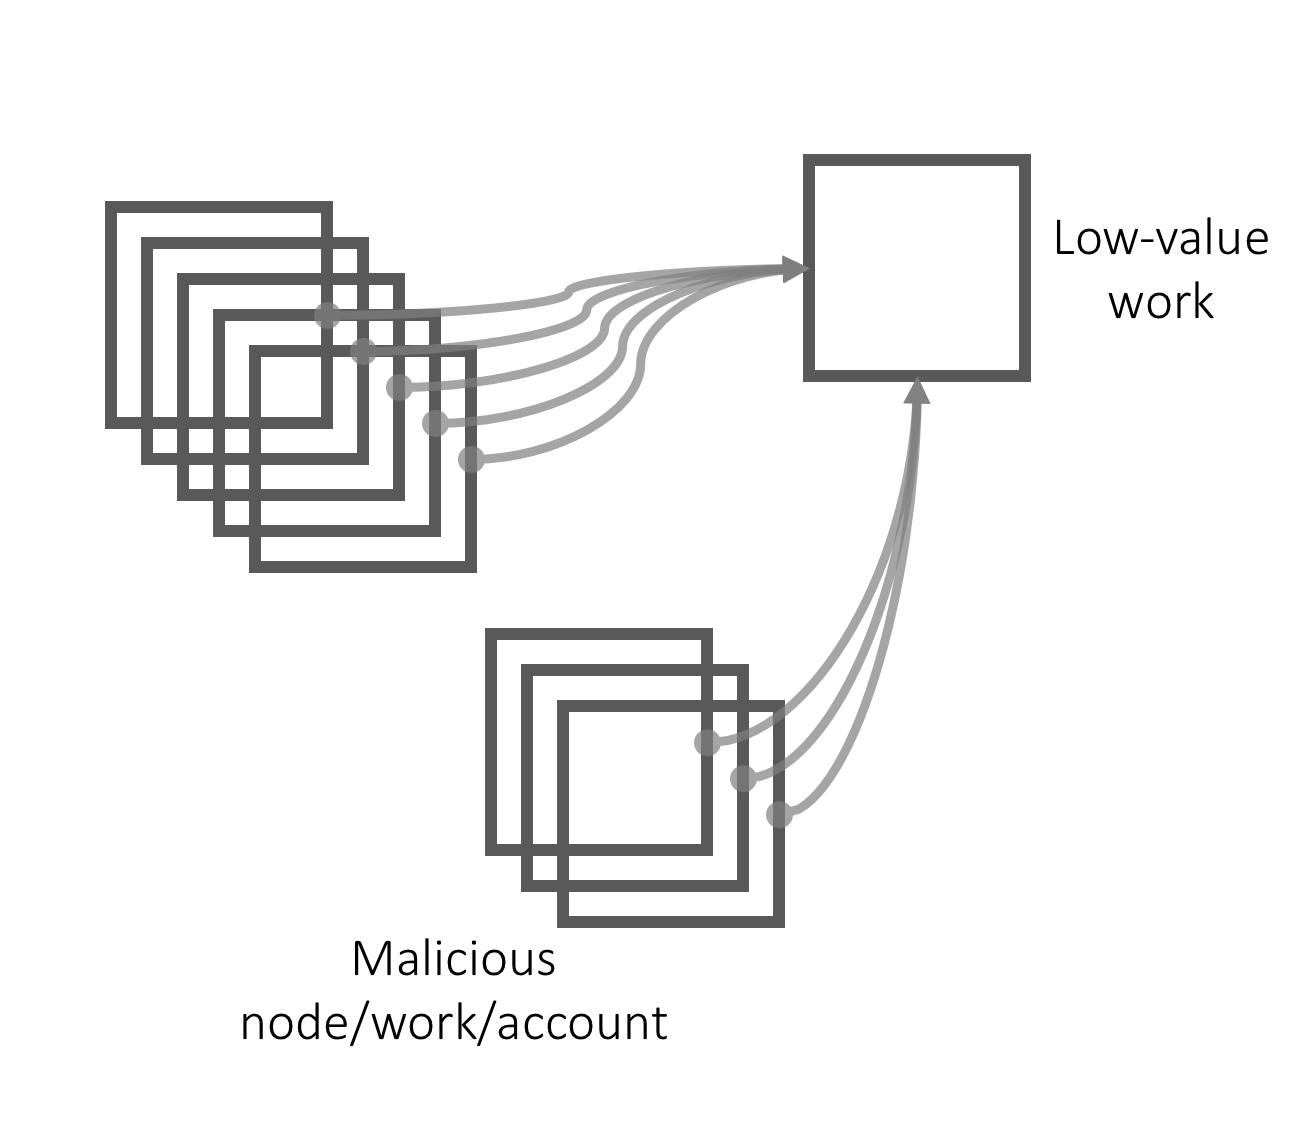
\includegraphics[width=\textwidth]{fig/lowV.png}
  \caption{Low-value Work. We regard "loop attack" as a subset of "Low-value work" attack. }
\end{marginfigure}






Assuming the existence of a completely worthless work, the author, by generating a large number of accounts, continuously cites the worthless work in order to deceive the reward of each block. This type of problem is the challenge of all the value judgment systems based on mutual citation. The performances of Random Walk Model and PageRank, NCDawareRank are basically the same, and they all avoid the massive storage consumption of decentralization. On the other hand, every citation is not completely free and the fee will be significantly higher than the general transaction. The current citation fee we set is equivalent to more than twice the normal transaction, and the amount of money transferred must be greater than or equal to the current transaction fee. In this case, for a malicious node, the number of citation cannot be too much, otherwise the deceived block award cannot make up for the fee resulting from citation itself.




\section{Retrospecctive Difficulty}

Bitcoin’s blockchain network generates about 50GB of data reach year and the size of our blockchain network will not significantly exceed this figure in early stages. For such a large data, the time consumed to search once will not be more than a few seconds. The honest miner can have the calculation difficulty greatly reduced only by complete search. The search difficulty should be in logarithmic growth without having a huge impact on the Random Walk Model itself.



Our goal is to bear all citation information of the academic journals and to award the outstanding works. When the amount of citation information of the block is quite large, the time for a single search may be extended to ten seconds or more. In this case, the miner will be likely to conduct only the first search (namely, find the location of the previous block, constant time consumption with the retrospective step being $1$). In this case, PoL and corresponding Random Walk Model will offer incentives for the search in terms of difficulty to attract the miners to re-search in the entire blockchain.

\section{Block Generation Time}
Compared to other digital currencies, the changes of the generation time of new block from the previous one will reach 50\% at most. But this is in a very extreme situation, and in most cases, the generation time will not exceed 10\%.





































%--------------------------------------
\chapter{Commercialization Program}




\section{Circulation of RCT}


The English for RCT program token is \emph{Reference and Certify Token} abbreviated as RCT with a total circulation of 420 million. The generation speed of the blockchain is 1m/block and the initial amount of block incentive is 50 token/block regularly halved. The consensus mechanism is PoW + PoI accounting for 60\% and 40\% respectively.




\begin{marginfigure}
  
\includegraphics[width=\textwidth]{fig/logo.png}
  \caption{The logo of Reference \& Certify Token}
\end{marginfigure}





\section{RCT Allocation Program}

The initial source of funding for the implementation of the project is mainly dependent on the support of ICO and early investors as well as public sale of the part of early investors and RCT community (50\%), etc. In the early stage of project implementation, this part of funds raised will be invested into model validation and network construction. Half of the 420 million token will be dug by the miners (give rewards in proportion according to PoW and PoI mechanisms). In the stage of promotion, 10\% of all flows will be used to finance academic research institutions and enterprises to participate in RCT network.









\begin{figure}
% Usage: \wheelchart{<value1>/<colour1>/<label1>, ...}
\wheelchart{210/RoyalBlue/"RCT Community",  84/WildStrawberry/"ICO", 84/Cyan/"Developers", 42/Black/"Finance the blockchain related research"}
\caption{RCT Allocation Program. (Unit: million)}
\end{figure}

































During the operation of the project, the creator needs to pay a certain RCT as a fee to establish a reference relationship (in order to prevent malicious establishment of the garbage reference). Once the reference relationship is established, 40\% of the RCT awarded will be rewarded to the "works" (wallet address) in the past block according to the its influence to encourage more people to join the citation chain and encourage creators to create more influential works. ICO and early investors can either choose to transfer RCT to others, or convert their works into a wallet address for others to cite to claim more RCT earnings.

\section{Milestones for the RCT Project}


Please refer Table \ref{timeMileS}.








\begin{table}
\label{timeMileS}
\caption{Timeline of RCT program}
\centering
% \begin{minipage}[t]{.7\linewidth}
\color{gray}
\rule{\linewidth}{1pt}
\ytl{Feb. 2017}{Preparation work for the citation chain project}
\ytl{Mar. 2017}{Early stage technical R\&D of the early founding team of the citation chain project}
\ytl{Sept. 2017}{ICO public flotation of the citation chain project}
\ytl{Nov. 2017}{Establishment of the prototype of the RCT project}
\ytl{Dec. 2017}{Public sale of RCT}
\ytl{Feb. 2018}{Public test of the citation chain}
\ytl{Aug. 2018}{Completion of the public test and online officially}
\bigskip
\rule{\linewidth}{1pt}%
% \end{minipage}%
\end{table}











%--------------------------------------
\chapter{Scenes of Application}


\section{Patent Conversion and Rapid Pricing of Scientific Research Products}


In the process of transformation of production, education and research, the industry needs to conduct quick and accurate pricing of scientific research products to meet the needs of a large number of highly efficient transformation research. In traditional research, peer review can be used to conduct a pricing study of a class of products to reflect the position of the research results throughout the research community. Based on the citation chain network, we will quantify the value judgments based on peer review and make the records unchangeable. When a work is introduced into a citation chain network, an account that has a higher reward in the industry (for example, an account that is constantly referenced in all previous nodes and has a high importance score) can be made simple for "reference", you can achieve the endorsement for the value of this product. One of the consequences of this is that the credit of the account becomes an important criterion for judging pricing and at the same time, the value of the work can be accounted for by the entire network.


\section{Research Paper/We-media/Blog/Network Literature}
The Internet is constantly reducing the cost of piracy, and authors of we-media/network literature and other original contents need to face the challenges of copyright infringement and other challenges without sufficient income. Although the citation chain network cannot achieve the task of recording the content itself, copyright verification is relatively simple for the works existing in the entire network own  hash value. This feature has also been proven by other blockchain networks.



\begin{figure}
  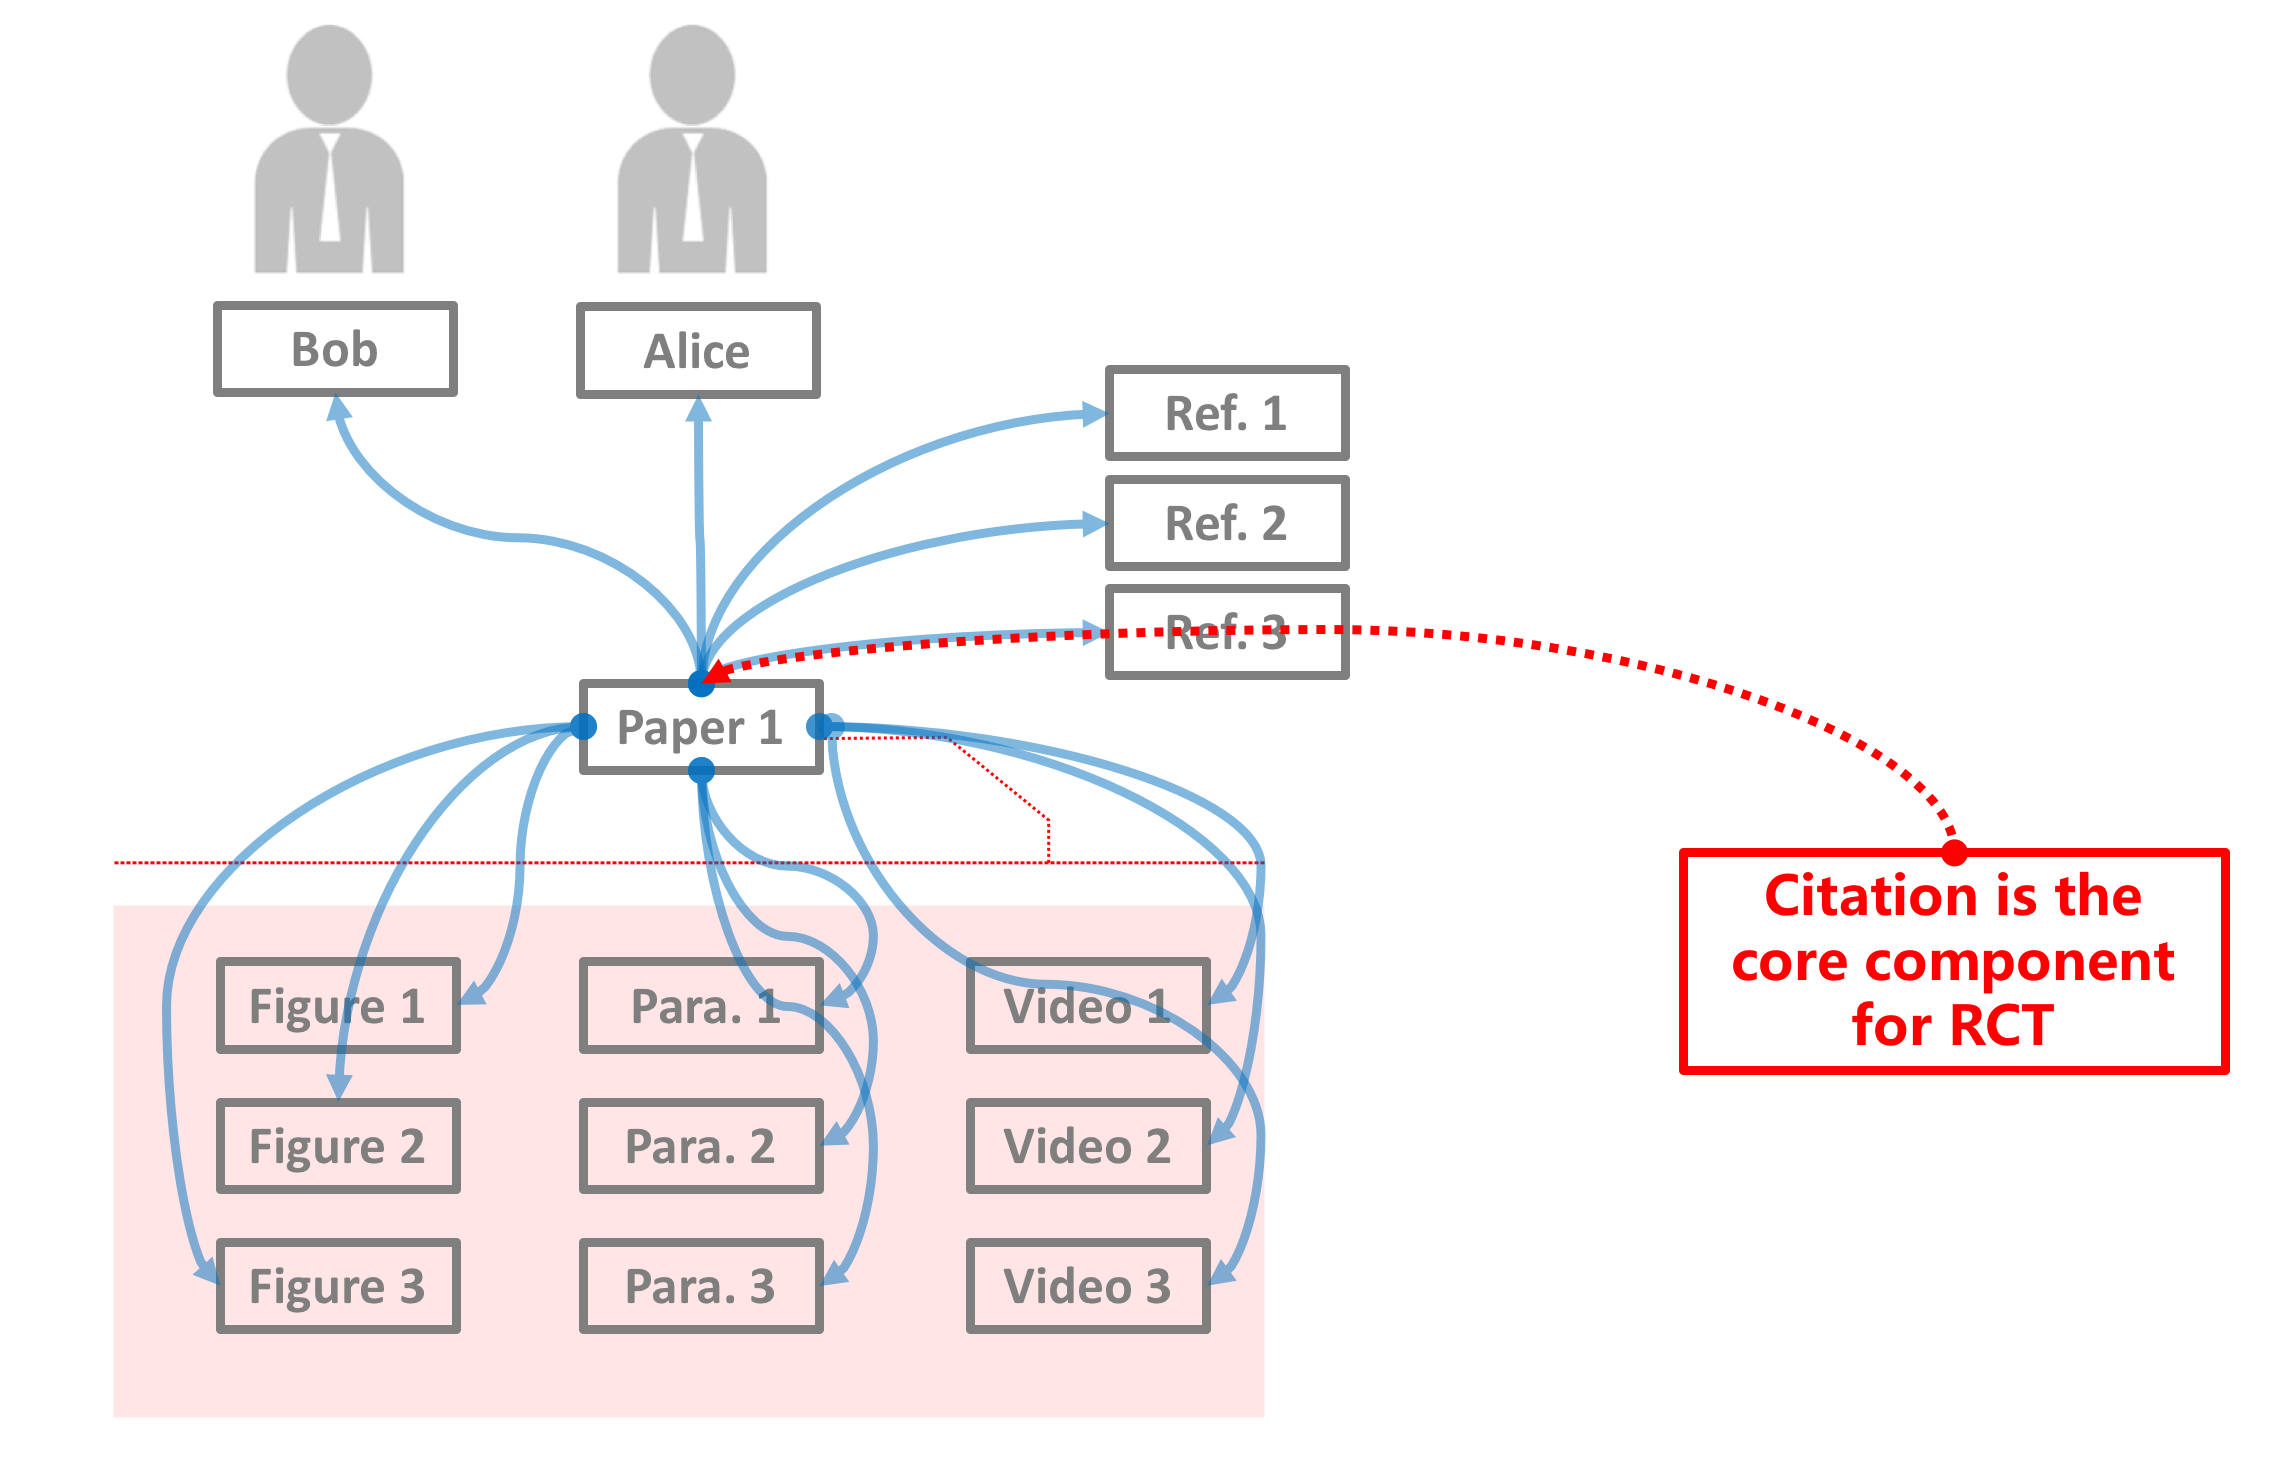
\includegraphics[width=\textwidth]{fig/bobAlice.png}
  \caption{An example of RCT application}
\end{figure}



One significant feature of the citation chain network differing from other blockchain networks is that systematic and scientific calculation has been done in terms of the awards of the original content of the network. Most of the modern social networks have cited the incentive mechanisms of "praise" and "opposition", and some platforms even judge the value of the entire work through the praise and opposition. But one of the challenges to this behavior is that a malicious node can generate massive virtual users in a short period of time to continually "praise" or "oppose" the work, thus affecting the platform's judgment of its value. The citation chain network, based on "citation" , conduct the value judgment, which on the one hand, costs the honest users a little for every "citation" with only a few transaction costs. But for a malicious node, if you want to deceive the network to obtain rewards, you need to generate massive users to repeat the "citation", so the income cannot even cover the required fee.


\begin{marginfigure}
  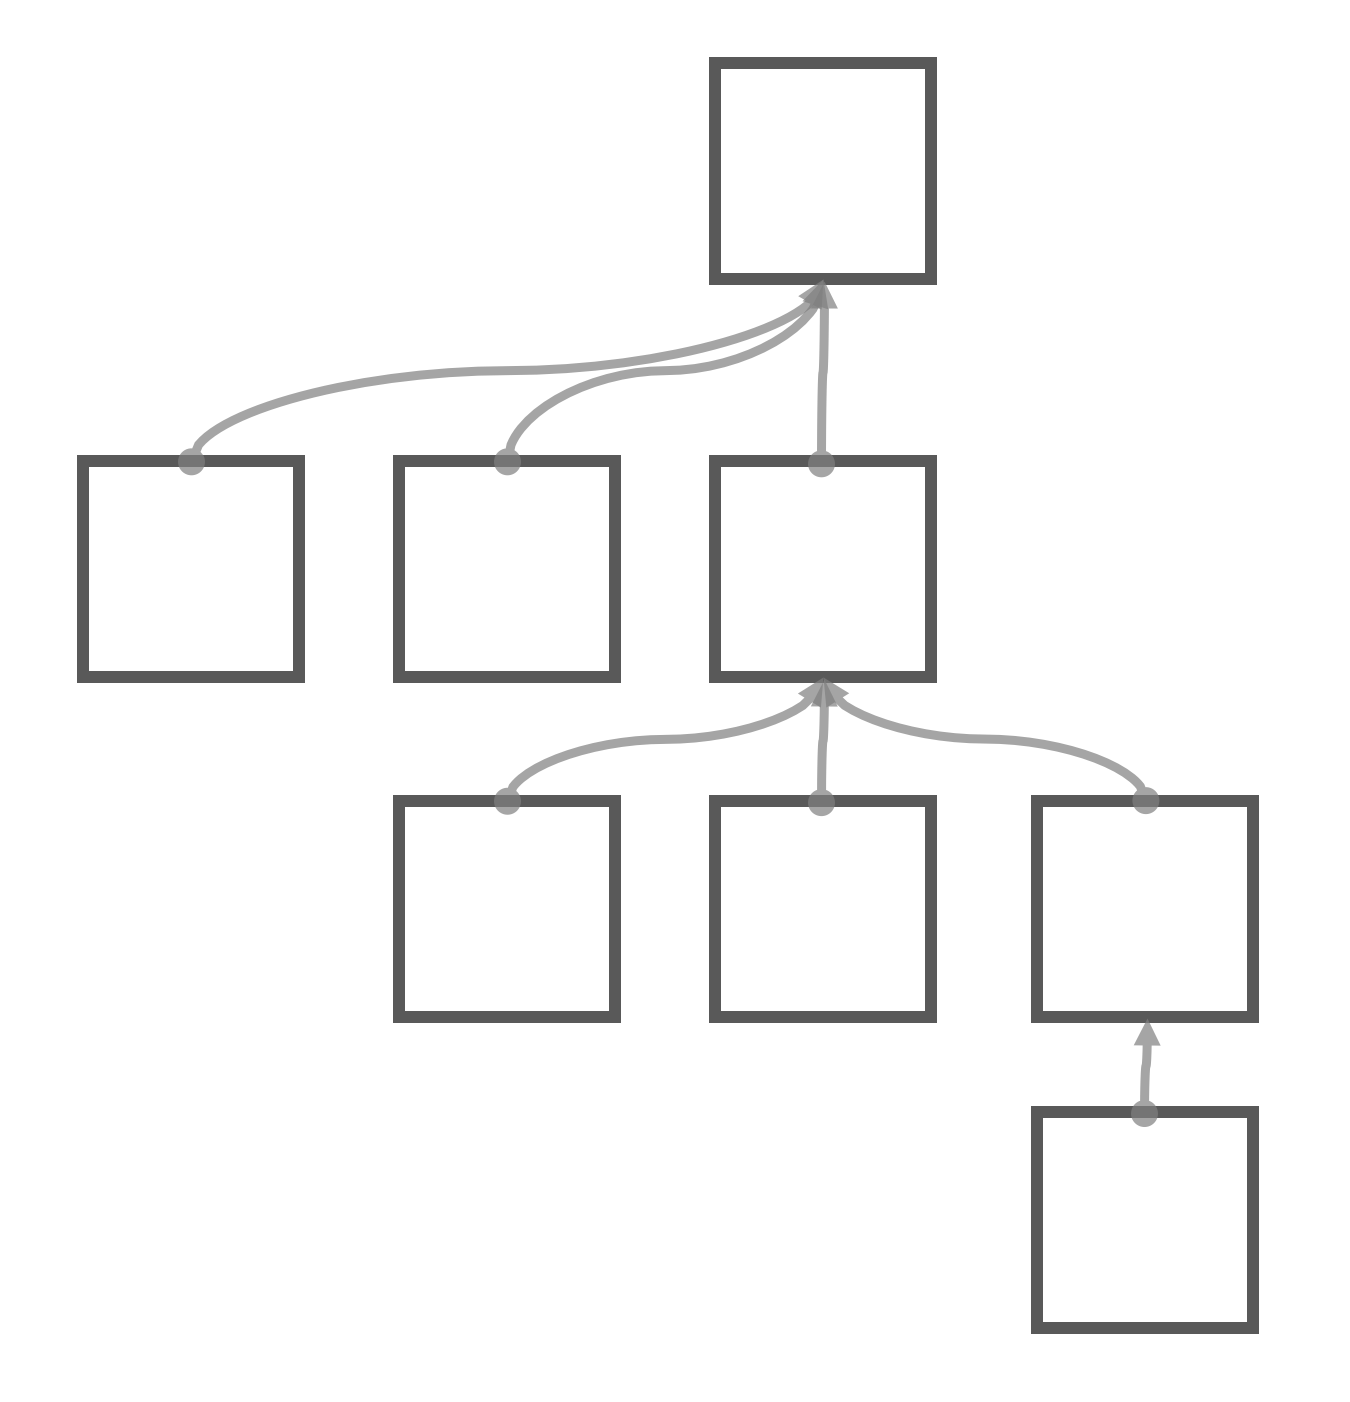
\includegraphics[width=\textwidth]{fig/treeC.png}
  \caption{Tree Citation: The way we recommend for citation structure. }
\end{marginfigure}

The author of the original works of the network can provide information such as the hash value, account address and other information in the website, social media, or the network platform we recommend to attract other authors to make a simple reward or more formal academic reference. For an original author, the cost of the above act is almost negligible, but it can be a lot of money by virtue of the value of his work.














%--------------------------------------
\chapter{Summary}


\begin{itemize}
  \item RCT can be used to create trustworthy value evaluation and transmission network;
  \item RCT network can bear all forms of creative works;
  \item The application of timestamp enables RCT network to realize property rights protection and copyright tracking effectively;
  \item By introducing an importance proof mechanism based on citation (PoI), RCT can judge the value of any work in a short period of time;
  \item The development of RCT project includes community construction, technical verification, token issuance and final network publishing;
  \item \textsf{\color{myQuote}{\textbf{\textit{\Large Our goal is to protect all intellectural property, reward and maintain the rights of global creators;}}}}



\end{itemize}




\end{document}








